\chapter{User in Smart Cities and new HMI}
\label{intro} 
\textsl{written by \\ Katrin Glöwing, matriculation number: 2170348} 
\\

\abstract{
This project is about controlling some system adjustments in the car by using hand gesture recognition.\\
For that project it is necessary to train a neuronal network and implement a program which uses the camera as an input device to recognise and detect the hand gestures.\\
This problem will be solved with an VGG-16 model with four additional dense layers on top and a cross-validation of two different data sets.\\
This program will help drivers to be more concentrated on the road and could also be an approach for intelligent systems which understands sign language.
}

\section{Introduction}
\label{sec:introduction}
In case of human machine interface is gesture control, means tending a hardware with gestures, particularly with hand gestures, growing in importance. The contact-free gesture control is aimed at a more intuitive interaction between user and machine \cite{Sommer2013}. Furthermore contact-free systems avoid the transmission of microbes. This is especially in the medical sector and in the care sector beneficial \cite{keiser2015gestensteuerung}.
\begin{figure}
\sidecaption
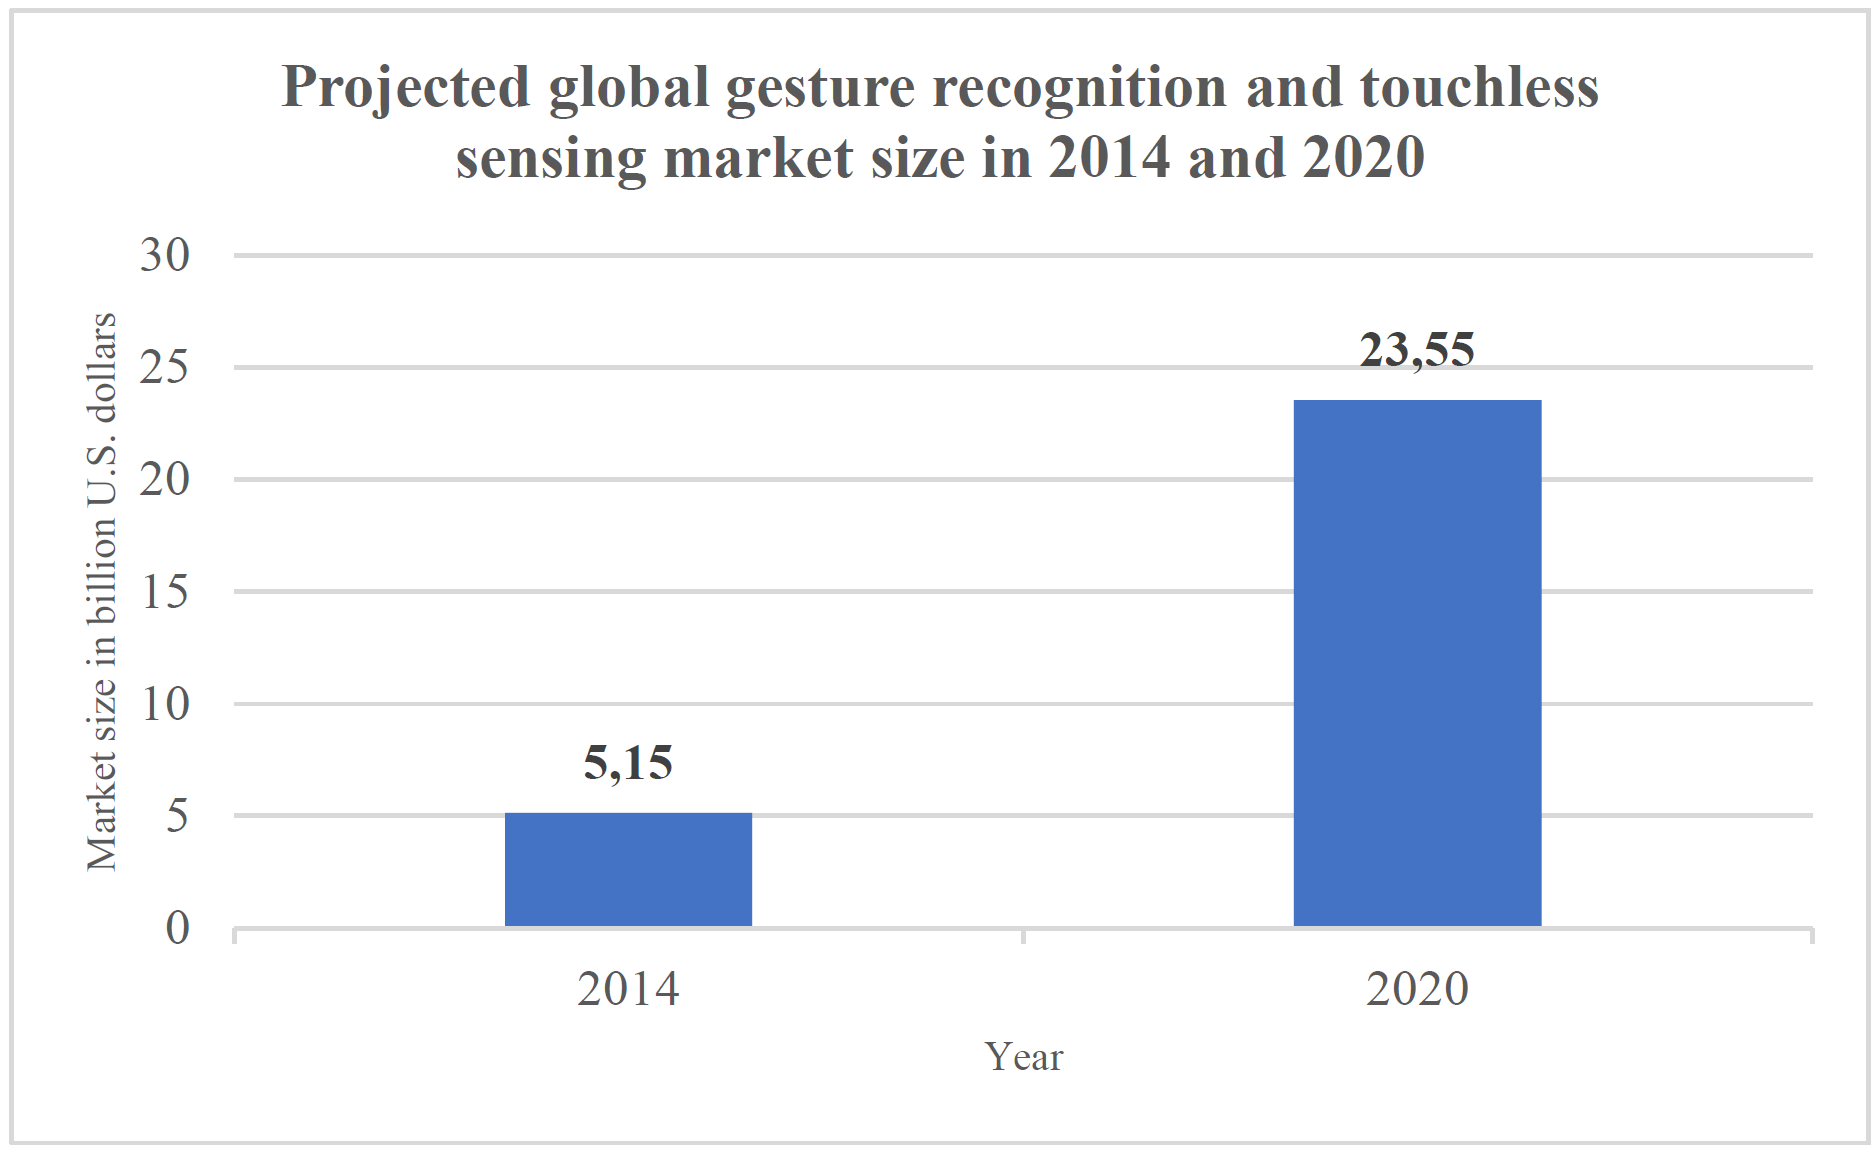
\includegraphics[scale=0.3]{images/gloewing_images/statistic_gesture_recognition.PNG}
\caption{Statistic: Projected global gesture recognition and touchless sensing market size \cite{statista2019}.}
\label{fig:statistic}
\end{figure}\\
Figure \ref{fig:statistic} compares the protected global gesture recognition and touchless sensing market size in 2014 and 2020. This statistic was published in 2014. As it is shown in Figure \ref{fig:statistic}, the market size worldwide was in year 2014 at 5,15 billion U.S. dollars while the projected market size in year 2020 is more than a quadruple of the size in 2014. The value of the projected global structure recognition and touchless sensing market amounts to 23,55 billion U.S. dollars.\\
The next section will presents some related works. The following section shows the concept including the goal, the requirements and the use cases. After that, the implementation is explained. First the used model and then follows some parts of the implementation with explanation. The results will be shown with the aid of a program showcase and by showing which of the before defined requirements are implemented. In the end there will be the conclusion including some potential future works and finally the references.


\section{Related works}
\label{sec:relatedworks}

Currently (2019) gesture control appears for example in the entertainment and the automotive sector. Until now is the gesture control among others recover in \textit{Microsoft Kinect} and \textit{Nintendo Wii} or also in TVs from \textit{Samsung} \cite{Courtney2019}.\\
With this hardware it is possible to control actions on the television screen or rather operate the TV by hand gestures from the user \cite{Courtney2019}.\\
In case of using gesture control in medical sector, it is possible to instruct robotic mechanism to perform complex surgical procedures by using hand gestures as commands \cite{medical1}. One approach, published in 2008, uses the hand gestures from the surgeons to take control over digital images. This means, it is possible to influence the digital images while an operation contact-free \cite{wachs2008gesture}.\\
In the automotive industry \textit{BMW} applies since 2016 in their \textit{7-er series} for example gesture control for diverse functions \cite{Courtney2019}.\\
This project corresponds to the automotive sector.



\section{Concept}
\label{sec:concept}
This report will explain a program for gesture recognition.

\subsection{Goal of the project}
\label{subsec:goal}
The goal of the project is to implement a system, which recognizes hand gestures from the user to control some system adjustments in the car.

\subsection{Requirements}
\label{subsec:requirements}
Figure \ref{fig:requirements} represents the requirements of this project. In summary there are seven requirements, four functional (Type: F) and tree non-functional (Type: NF) requirements.\\
Functional requirements are requirements which describes what a system or product must execute \cite{robertson2012mastering} and non-functional requirements describes the fundamental basics of the systems architecture \cite{6365165}.
\begin{figure}
\sidecaption
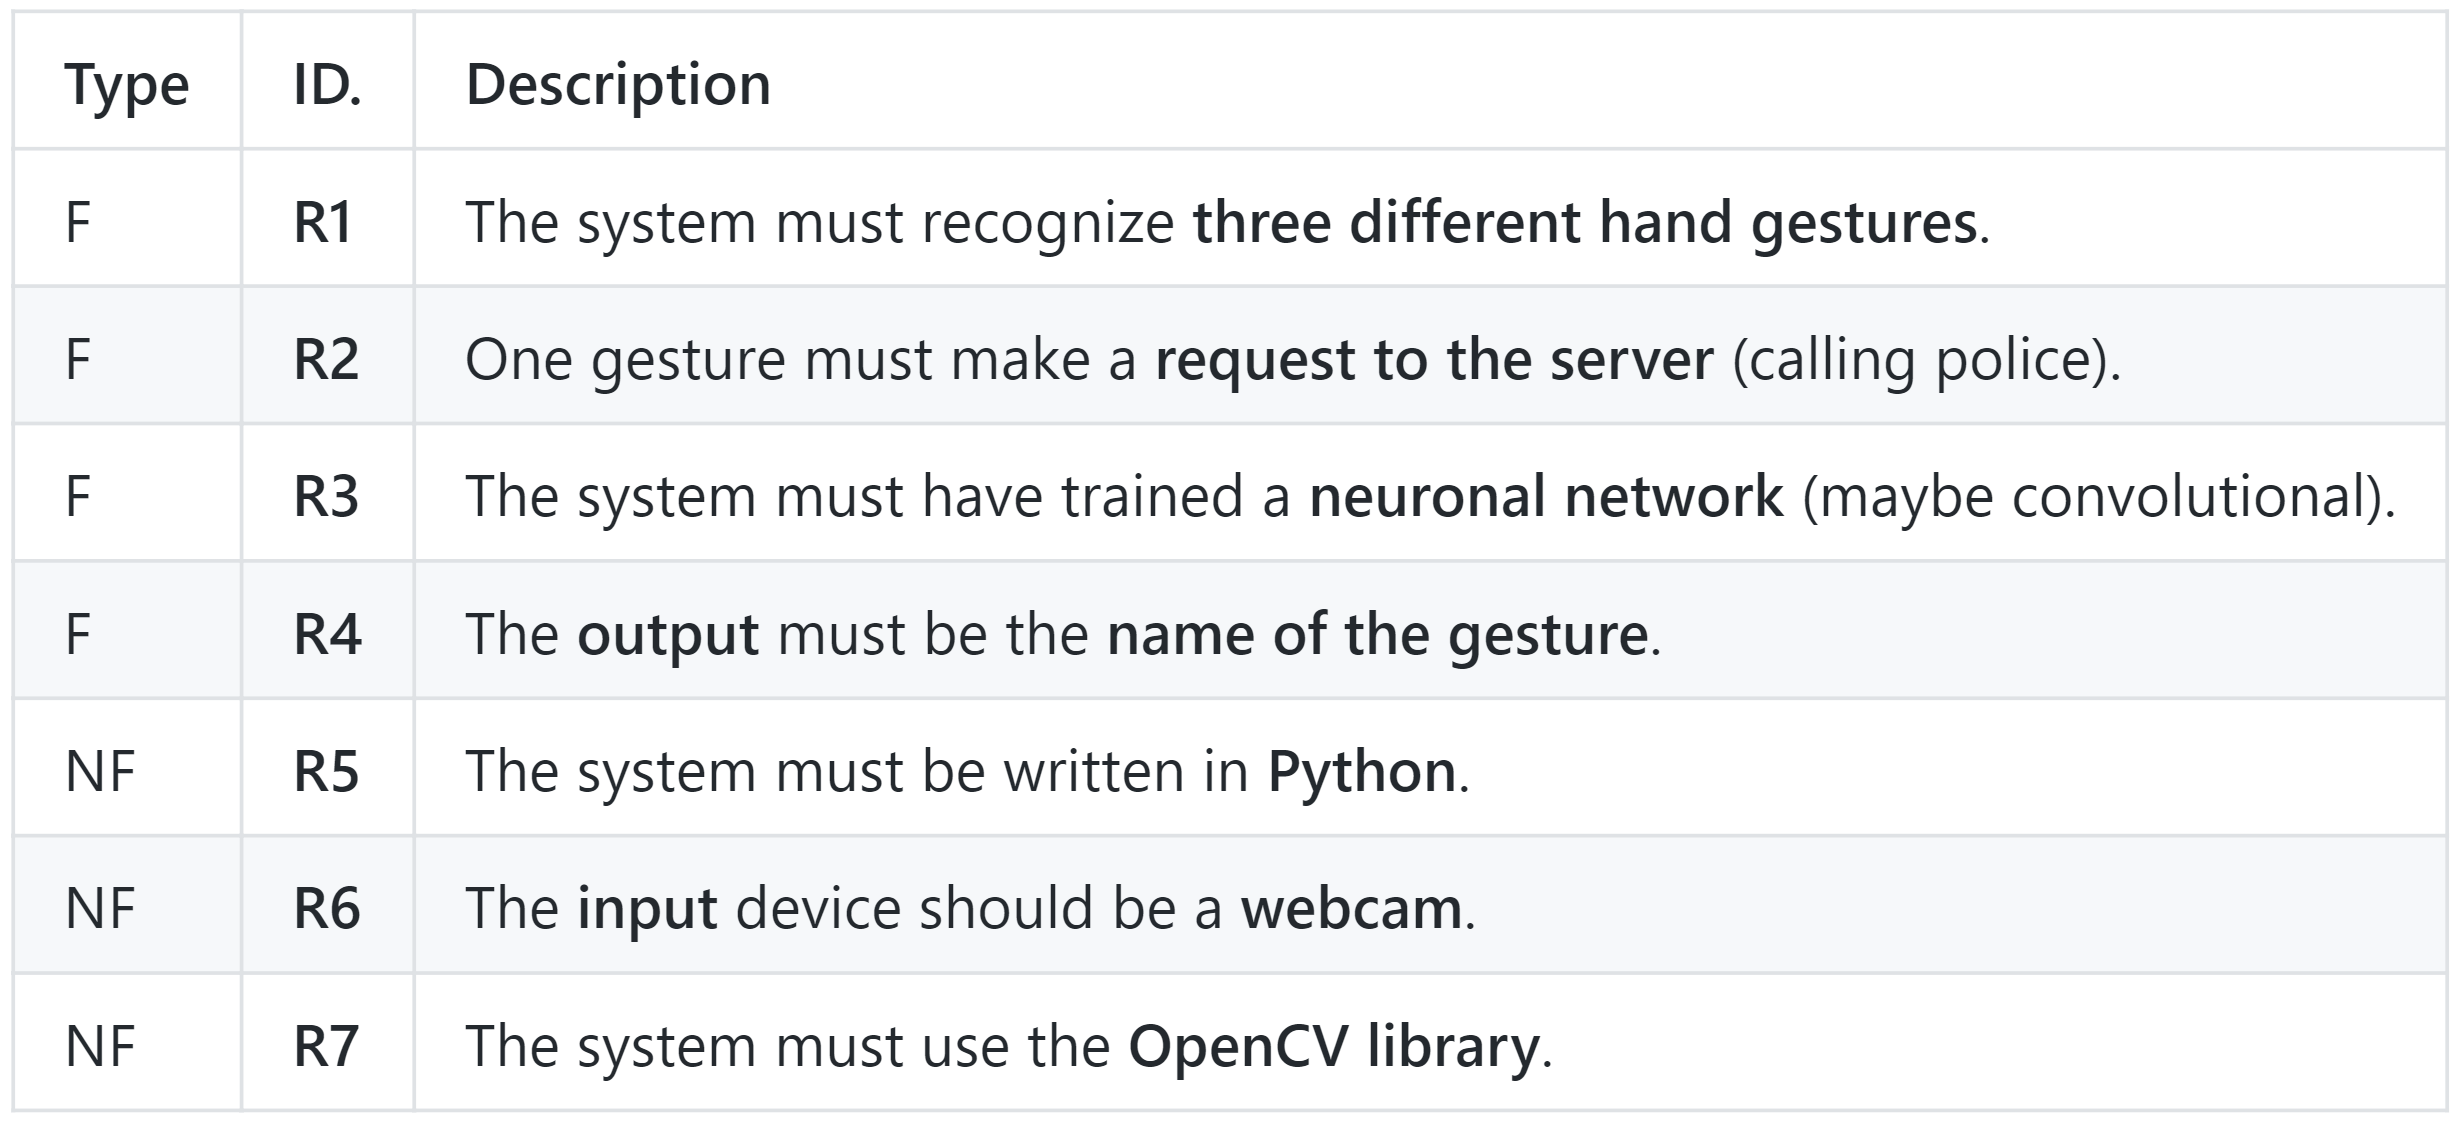
\includegraphics[scale=0.23]{images/gloewing_images/requirements.PNG}
\caption{Requirements of the project.}
\label{fig:requirements}
\end{figure}\\
The system must recognise three different hand gestures (ID.: R1) and show the name of the identified gesture (ID.: R4) by using a webcam as an input device (ID.: R6). One of these gestures must makes a request to the server to call the police (ID.: R2). The system must have trained a neuronal network (ID.: R3), must be written in the program language Python (ID.: R5) and must use the OpenCV library (ID.: R7).


\subsection{Use Cases}
\label{subsec:usecases}
Figure \ref{fig:usecase} shows the UML Use Case Model of the project. The project has three actors: the \textit{car driver}, the \textit{gesture recognition system} and the \textit{server} of the smart city.\\
The process is each time similar. The car driver \textit{performs a hand gesture} and this includes that the gesture recognition system \textit{recognizes the hand gesture} and runs the connected command. For example, when the car driver \textit{performs the hand gesture "Fist"}, the gesture recognition system \textit{recognizes the hand gesture "Fist"} and \textit{turns the music on}.\\
One use case is connected to the server. If the car driver \textit{performs hand gesture "L"}, the system \textit{recognizes hand gesture "L"} and \textit{calls the police}, the system will be \textit{connected to the server} and will \textit{send user data and reason (police) to the server}. The specified reason is the reason why the system would request to the server. The server \textit{receives the data} and \textit{replies to the system}. These answer could be \textit{the distance value}, when everything works and the communication is successfully or otherwise an \textit{error}.
\begin{figure}
\sidecaption
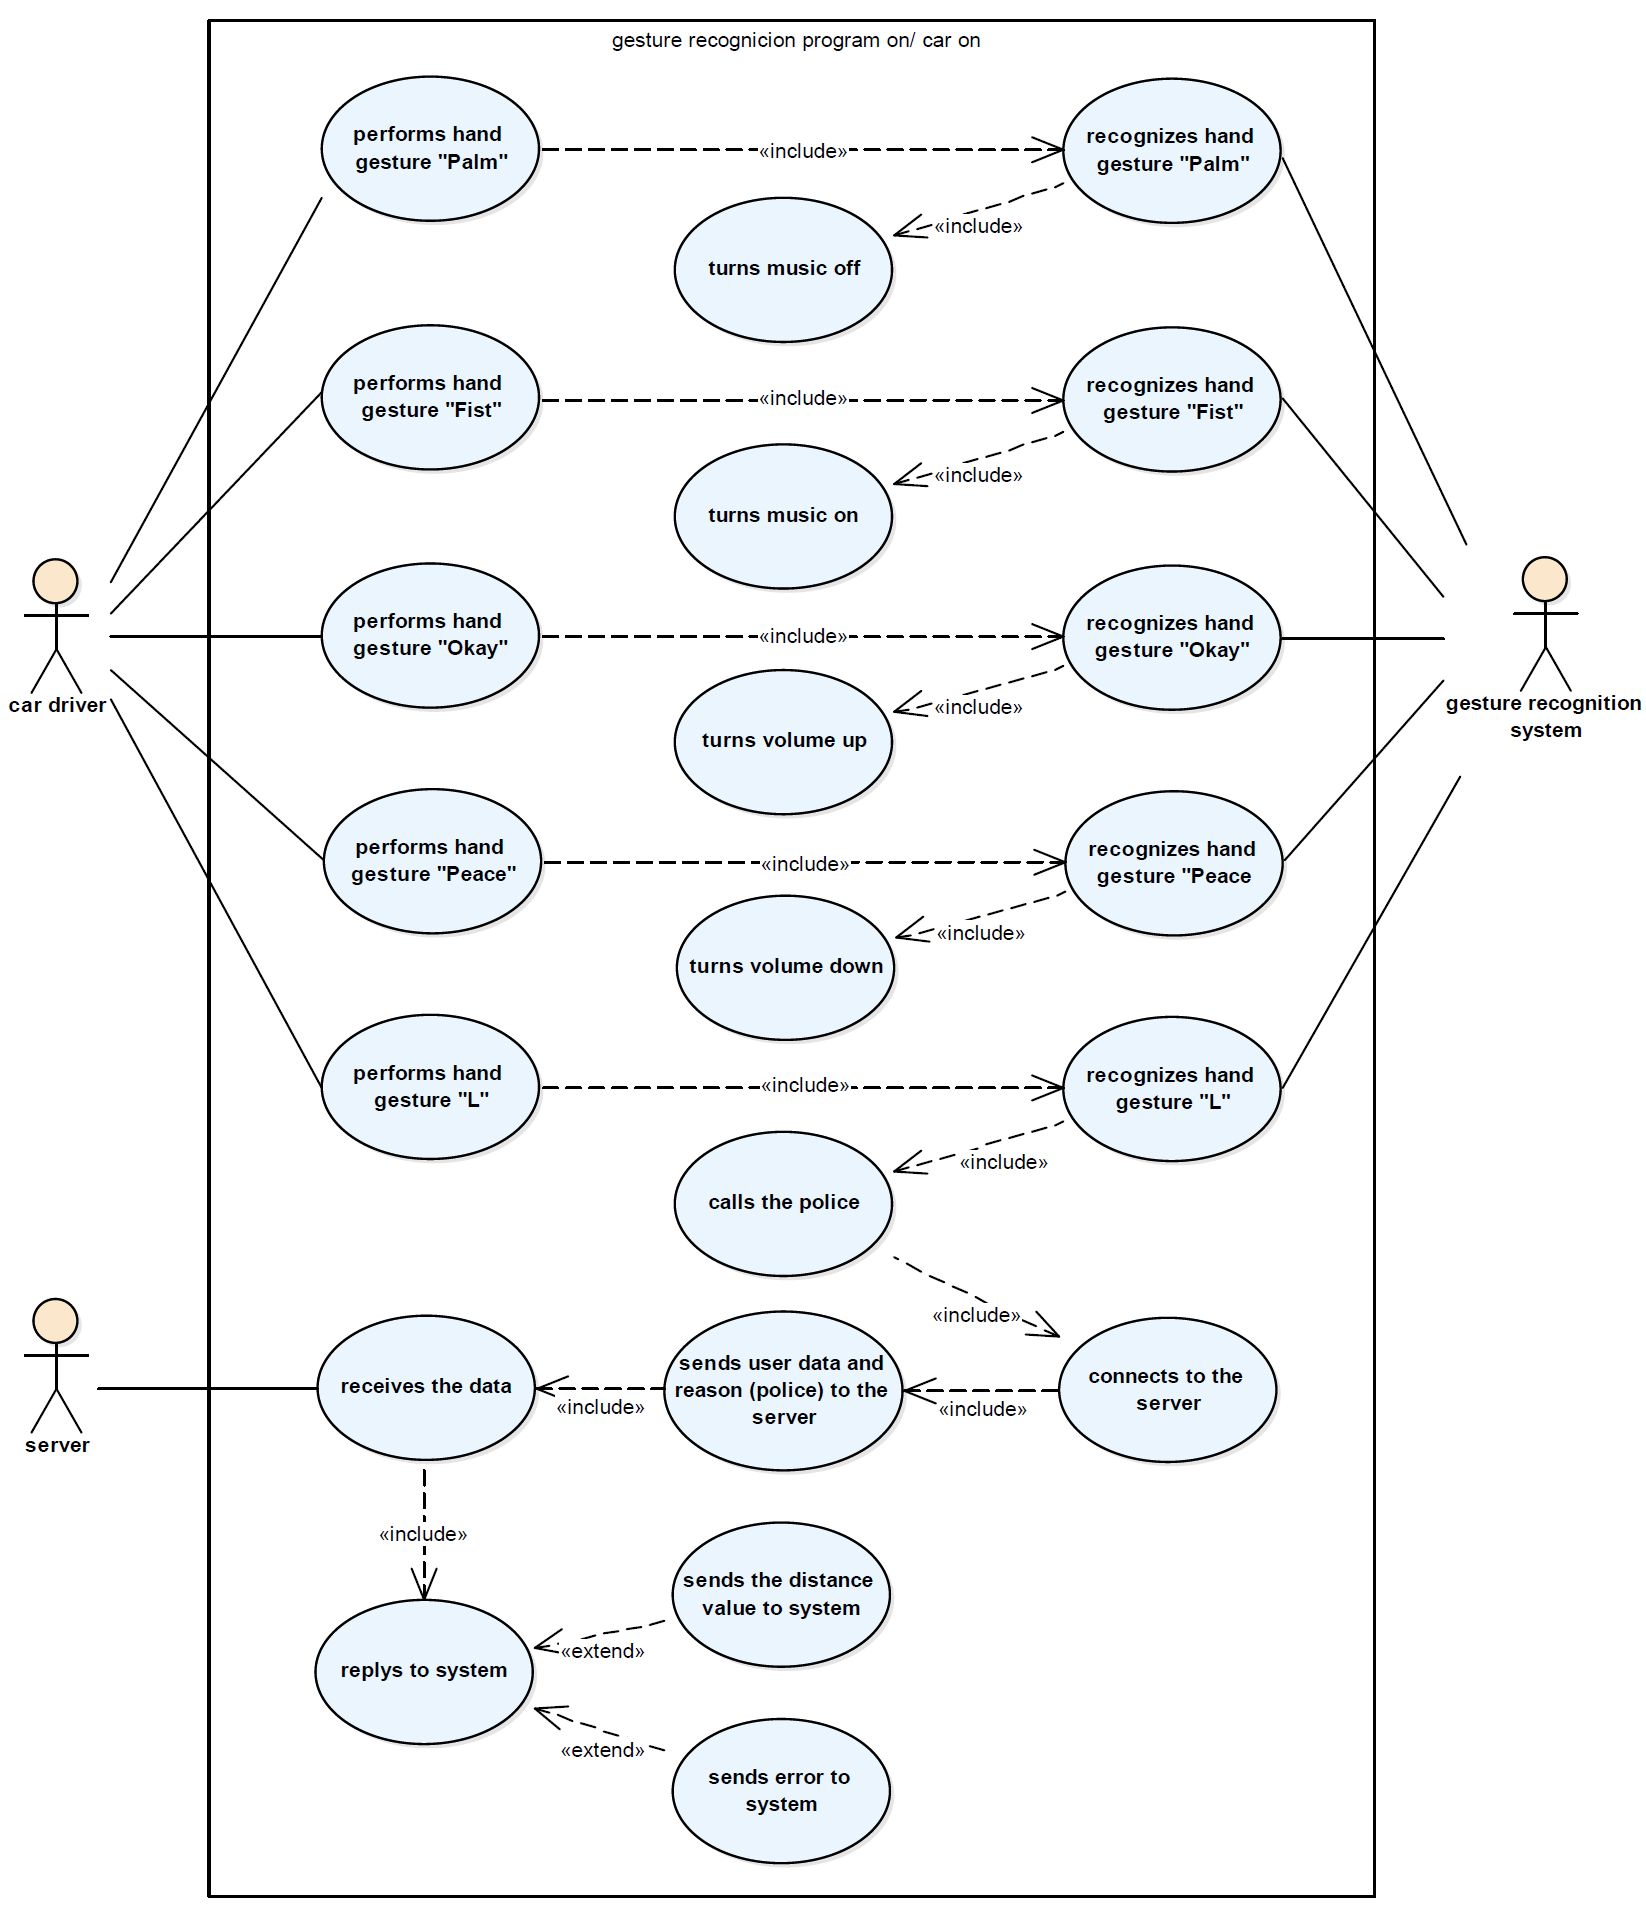
\includegraphics[scale=0.6]{images/gloewing_images/Usecases.PNG}
\caption{Use Case Model.}
\label{fig:usecase}
\end{figure}


\section{Implementation}
\label{sec:implementation}

\subsection{VGG-16 Model}
\label{subsec:vgg16}
The system uses the VGG-16 pre-trained model. The model is published in 2014 by Karen Simonyan and Andrew Zisserman in "Very Deep Convolutional Networks for Large-Scale Image Recognition" \cite{simonyan2014deep}. This model is a convolution neural net which enables handling a matrix, especially pictures which are painted as a matrix, as an input. Handling a matrix as an input has the advantage that the system is capable of recognizing idem objects as the same objects no matter in which position they are in the picture \cite{Becker2019}.
\begin{figure}
\sidecaption
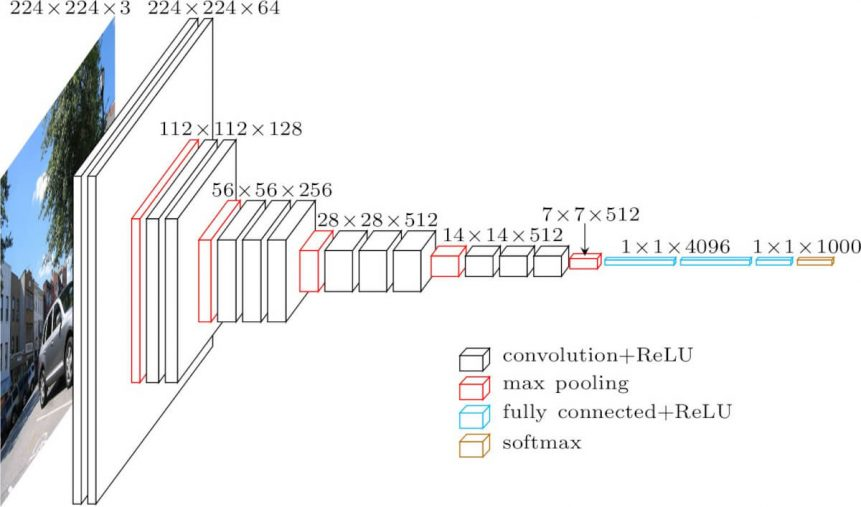
\includegraphics[scale=0.3]{images/gloewing_images/vgg16.png}
\caption{Architecture of the VGG-16 Model \cite{Hassan2018}.}
\label{fig:vgg16}
\end{figure}\\
Figure \ref{fig:vgg16} shows the architecture of the used VGG-16 model. As you can see on the left side of the picture, the model needs 224x224 RGB image as an input. The third value is the number of channel of 3x3 kernel of the convolution layer \cite{Hassan2018}.\\
A pile of convolution layers were traversed by the input image. The smallest receptive field size (3x3) to capture the outline sides and the center is used in this filters \cite{Hassan2018}.\\
The first steps are two \textit{convolution layers} followed by one \textit{max pooling layer}. Then again two \textit{convolution layers} followed by one \textit{max pooling layer}. After that follows three \textit{convolution layers} and one \textit{max pooling layer}. The next layers are three \textit{convolution layers} and one \textit{max pooling layer} and again three \textit{convolution layers} and one \textit{max pooling layer}. Summarised the sequence that the model follows is, using multiple convolution layers (Figure \ref{fig:vgg16}, black layers), two or three, and after that max pooling (Figure \ref{fig:vgg16}, red layers) has to be done. The size of the picture is quickly getting reduce. It starts at 224, minimize next to 112, than it comes to 56, next 28, than 14 and finally the size of the picture is 7. Then follows three \textit{fully connected dense layers} \cite{Hassan2018}.\\
The size of the image is reducing because of the max pooling layers. These layers have the pool stride of 2, which means the size of this layers is 2x2 and this is the reason why the image size will be bisected every time after the max pooling layer \cite{Hassan2018}.\\
The three consecutive \textit{fully connected layers} (Figure \ref{fig:vgg16}, blue layers) collects the outputs of the previous \textit{convolution layers} and \textit{pooling layers}. In these \textit{dense layers} is everything connected to each single input and output \cite{Becker2019}.\\
Convolution layers and fully connected layers were brought into action through the \textit{ReLU function}. This function raises each value which is below zero to zero and does not change each value which is higher than zero. Thereby is a better gradient propagation given. If this is not given and the vanishing gradient problem exist, it could be that the neuronal network will stop the further training \cite{Becker2019}.\\
The last layer, the \textit{softmax layer} (\ref{fig:vgg16}, yellow layer), results in a sum total of one by summing up all the previous outputs. This softmax layer also indicate the particular probability, if the class is true or false, of the outputs \cite{Becker2019}.


\subsection{Gesture Recognition System}
\label{subsec:system}
The implementation of this project is written in Python and uses the OpenCV library \cite{Brenner2018}.
\begin{figure}
\sidecaption
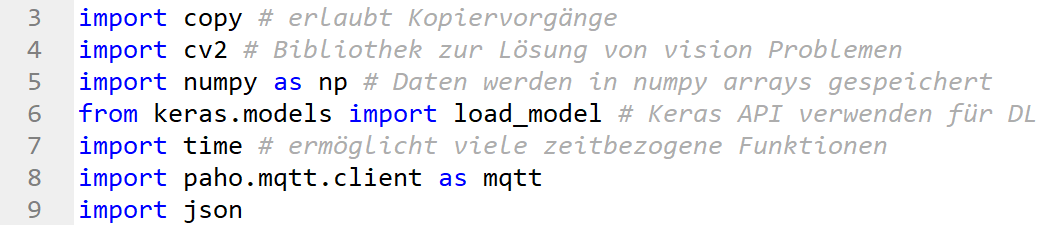
\includegraphics[scale=0.54]{images/gloewing_images/import.PNG}
\caption{Importing the necessary packages \cite{Brenner2018}.}
\label{fig:import}
\end{figure}\\
At first all the necessary packages has to be imported, as it is shown in Figure \ref{fig:import} \cite{Brenner2018}:
\begin{itemize}
    \item The system needs \textit{copy} to allow copy processes \cite{Brenner2018}.
    \item \textit{Cv2} is a library which solves vision problems and is used in our program among other things for using the camera and the keyboard \cite{Brenner2018}.
    \item With the \textit{numpy as np} importation it is possible to save the images as arrays, in this case in arrays with three channel (RGB) \cite{Brenner2018}.
    \item The \textit{keras.models import model} command, makes it possible to load and use the VGG-16 model \cite{Brenner2018}.
    \item The \textit{time} importation brings a lot of time functions with it \cite{Brenner2018}.
    \item \textit{Paho.mqtt.client as mqtt} is needed to connect this system to the local mqtt broker.
    \item With the importation of \textit{json} is it possible to connect this system to the server and to send and receive data from the server.
\end{itemize}
\begin{figure}
\sidecaption
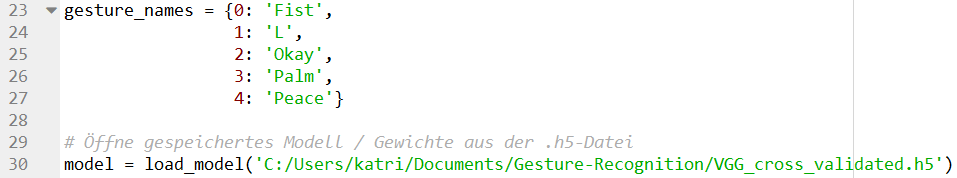
\includegraphics[scale=0.6]{images/gloewing_images/names_model.PNG}
\caption{Defining the gesture names and loading the model \cite{Brenner2018}.}
\label{fig:names_model}
\end{figure}
Figure \ref{fig:names_model} shows the determination of the gesture names and the command that loads the used model \cite{Brenner2018}.\\
There will be five gestures: \textit{fist}, \textit{L}, \textit{Okay}, \textit{Palm} and \textit{Peace}. In section \ref{sec:results} are the associated pictures of this gesture names \cite{Brenner2018}.\\
The used \textit{model} is the already explained VGG-16 Model (see section \ref{subsec:vgg16}) with four additional dense layers on top \cite{Brenner2018}.
\begin{figure}
\sidecaption
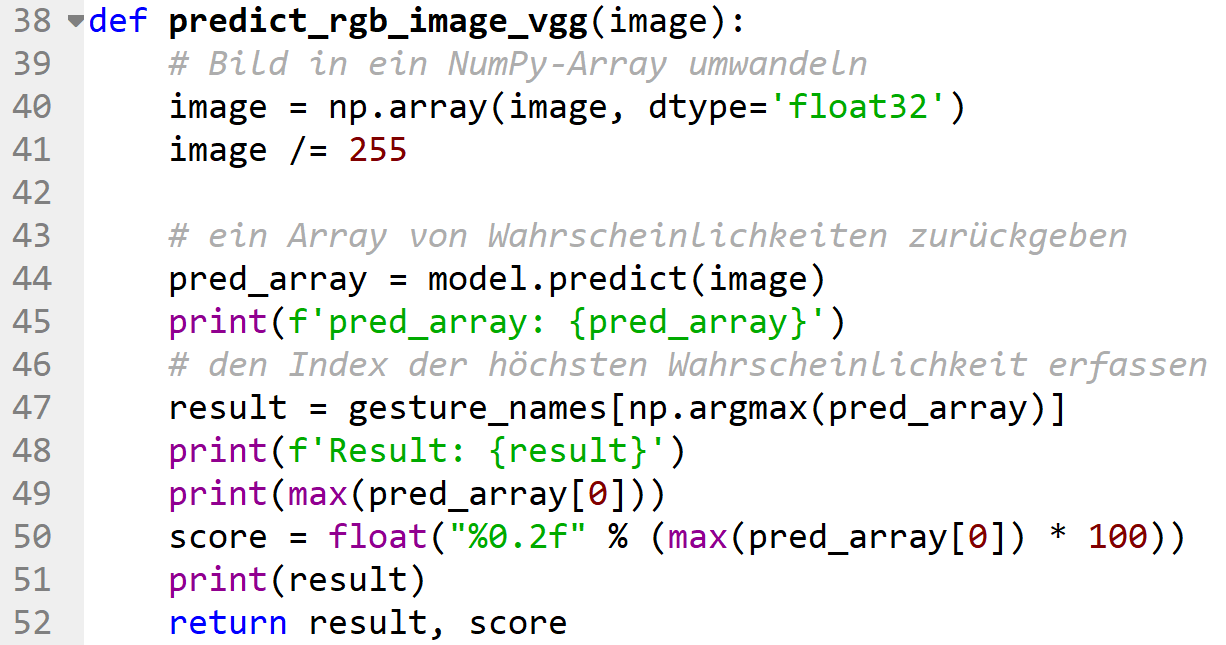
\includegraphics[scale=0.4]{images/gloewing_images/prediction.PNG}
\caption{Transforming the data \cite{Brenner2018}.}
\label{fig:predict}
\end{figure}\\
Figure \ref{fig:predict} shows the function \textit{predict\_rgb\_image\_vgg(image)} which is used to transform the data. The image is grabbed from the screen and resized. The model has to understand the input and that is why the image is transformed into a NumPy array in the next step \cite{Brenner2018}.\\
\begin{figure}
\sidecaption
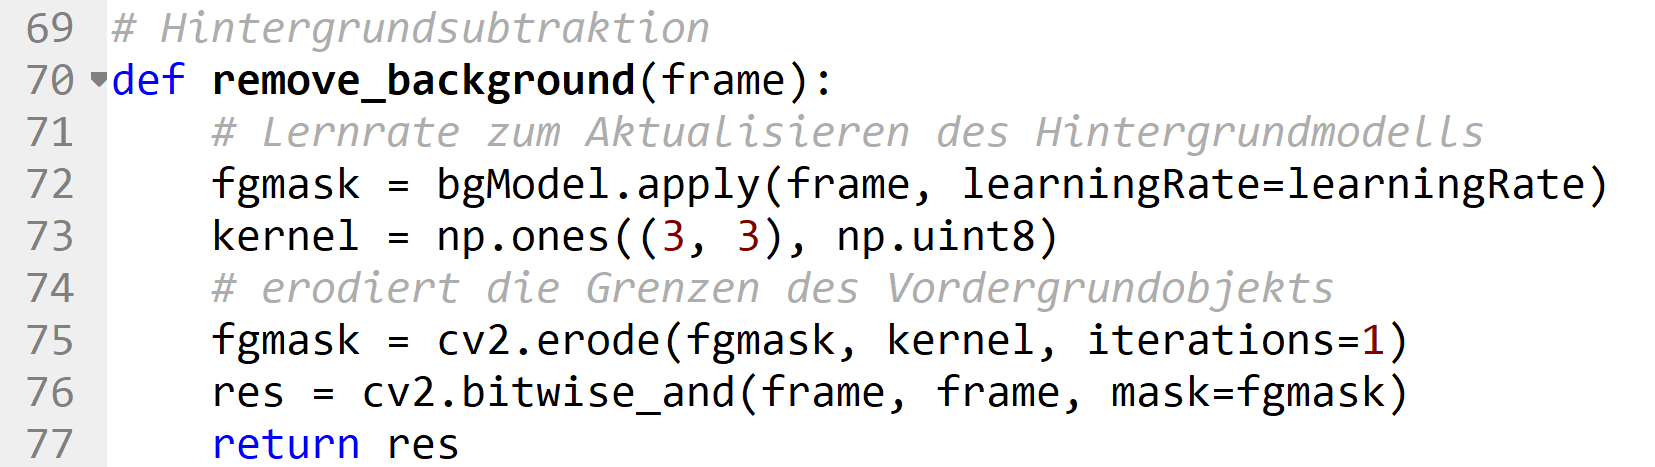
\includegraphics[scale=0.3]{images/gloewing_images/remove_background.PNG}
\caption{Extracting the gesture \cite{Brenner2018}.}
\label{fig:remove_background}
\end{figure}\\
To recognize the gesture it is necessary to subtract the background\\ (\textit{remove\_background(frame)}) as it is shown in Figure \ref{fig:remove_background}. First step is to create a mask (\textit{fgmask}) of the background by capturing the background before the hand of the user is in the frame. If the user now appears his or her hand in the frame, the mask will only show the hand and eliminate everything else \cite{Brenner2018}.\\
The next step, also shown in Figure \ref{fig:remove_background}, is to change the background to black and the hand, which is what the system should analyze, to white by using binary threshold values. This is necessary to recognize every hand, no matter which skin color the hand has and also for using this program with colourful gloves. This step is also needful to extract the gesture from the background clearly \cite{Brenner2018}. 
\begin{figure}
\sidecaption
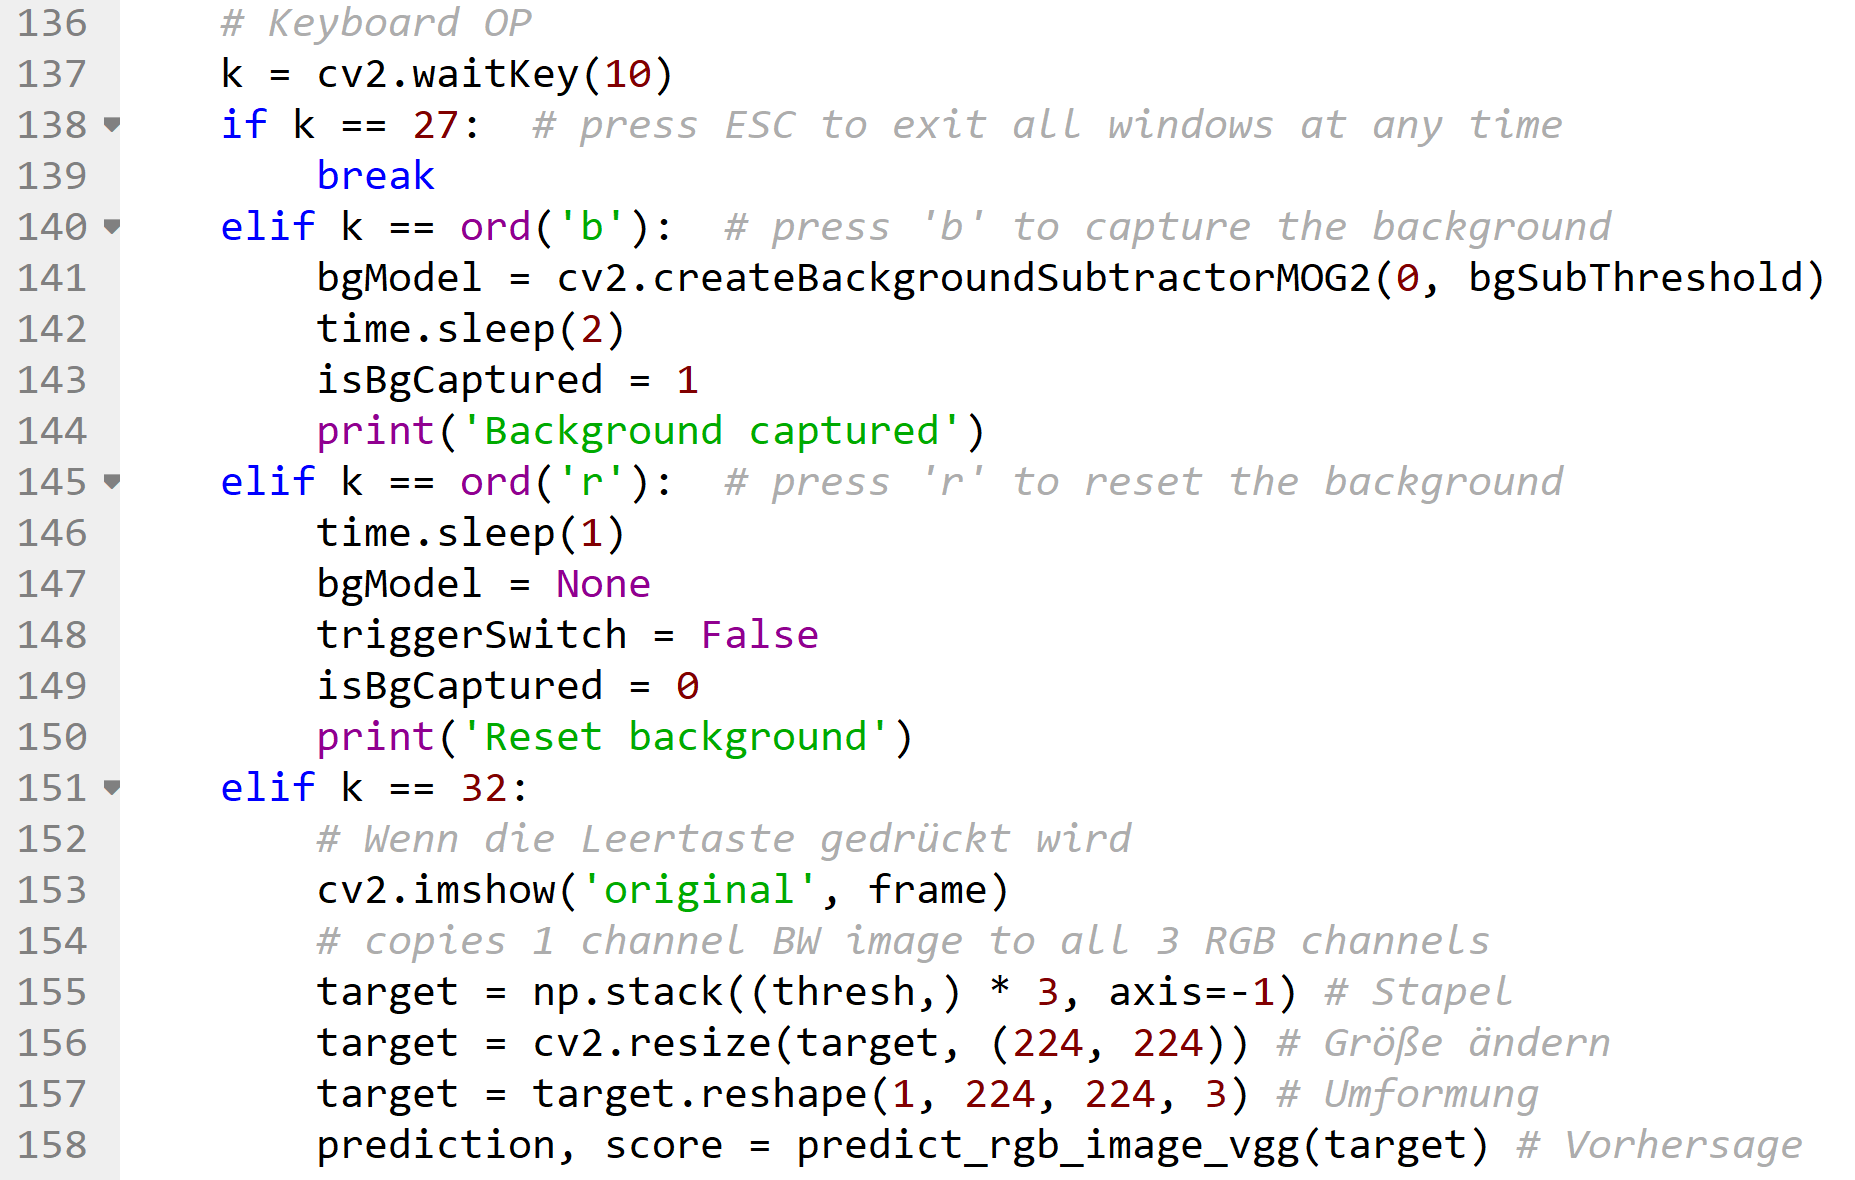
\includegraphics[scale=0.3]{images/gloewing_images/keyboard.PNG}
\caption{Using the keyboard to control the system \cite{Brenner2018}.}
\label{fig:keyboard}
\end{figure}\\
While the camera is open, which means also while the system is running, the user can control the system with the keyboard. The shortcuts were defined in Figure \ref{fig:keyboard} \cite{Brenner2018}:
\begin{itemize}
    \item If the user presses the escape key (\textit{if k == 27}), all the windows will be exit at any time \cite{Brenner2018}.
    \item If the user presses the b-button on the keyboard (\textit{k == ord('b')}), the background will be captured \cite{Brenner2018}.
    \item When the r-button will be pressed (\textit{k == ord('r')}), the system will reset the background \cite{Brenner2018}.
    \item When the space-bar will be pressed by the user, the output will be the recognized gesture \cite{Brenner2018}.
\end{itemize}
There is also one option, which is not shown in Figure \ref{fig:keyboard}, to turn the tracker on. This is for expanding the data set \cite{Brenner2018}.
\begin{figure}
\sidecaption
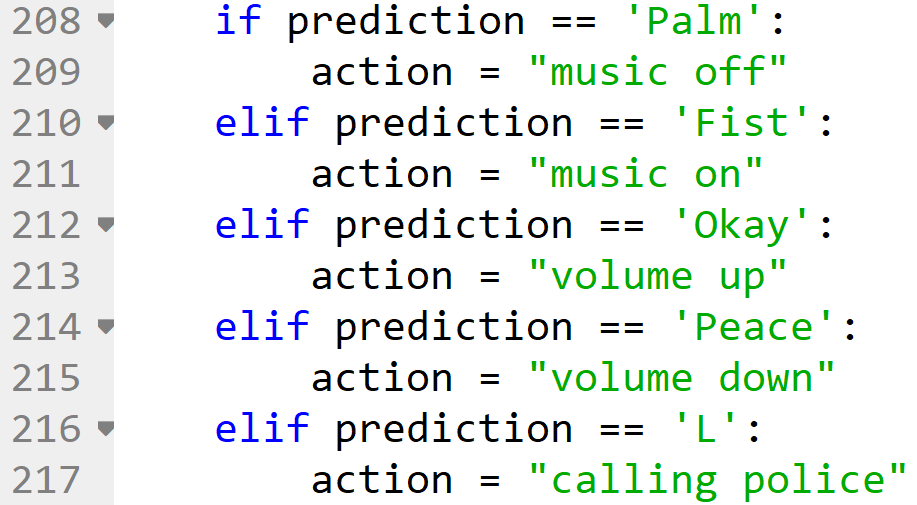
\includegraphics[scale=0.4]{images/gloewing_images/prediction_action.PNG}
\caption{Defining the corresponding actions of the well defined gestures \cite{Brenner2018}.}
\label{fig:predict_action}
\end{figure}\\
Figure \ref{fig:predict_action} shows what the system does when the gesture is recognized \cite{Brenner2018}:
\begin{itemize}
    \item If the prediction is \textit{'Palm'}, the system will turn the music in the car off \cite{Brenner2018}.
    \item If the prediction of the gesture is \textit{'Fist'}, the system will turn the music on \cite{Brenner2018}.
    \item If the system predict the gesture \textit{'Okay'}, the volume will be turned up \cite{Brenner2018}.
    \item If the prediction is \textit{'Peace'}, the volume will be turned down \cite{Brenner2018}.
    \item If the system predict the gesture \textit{'L'}, the police will be called by connecting this system to the server of the smart city.
\end{itemize}
\begin{figure}
\sidecaption
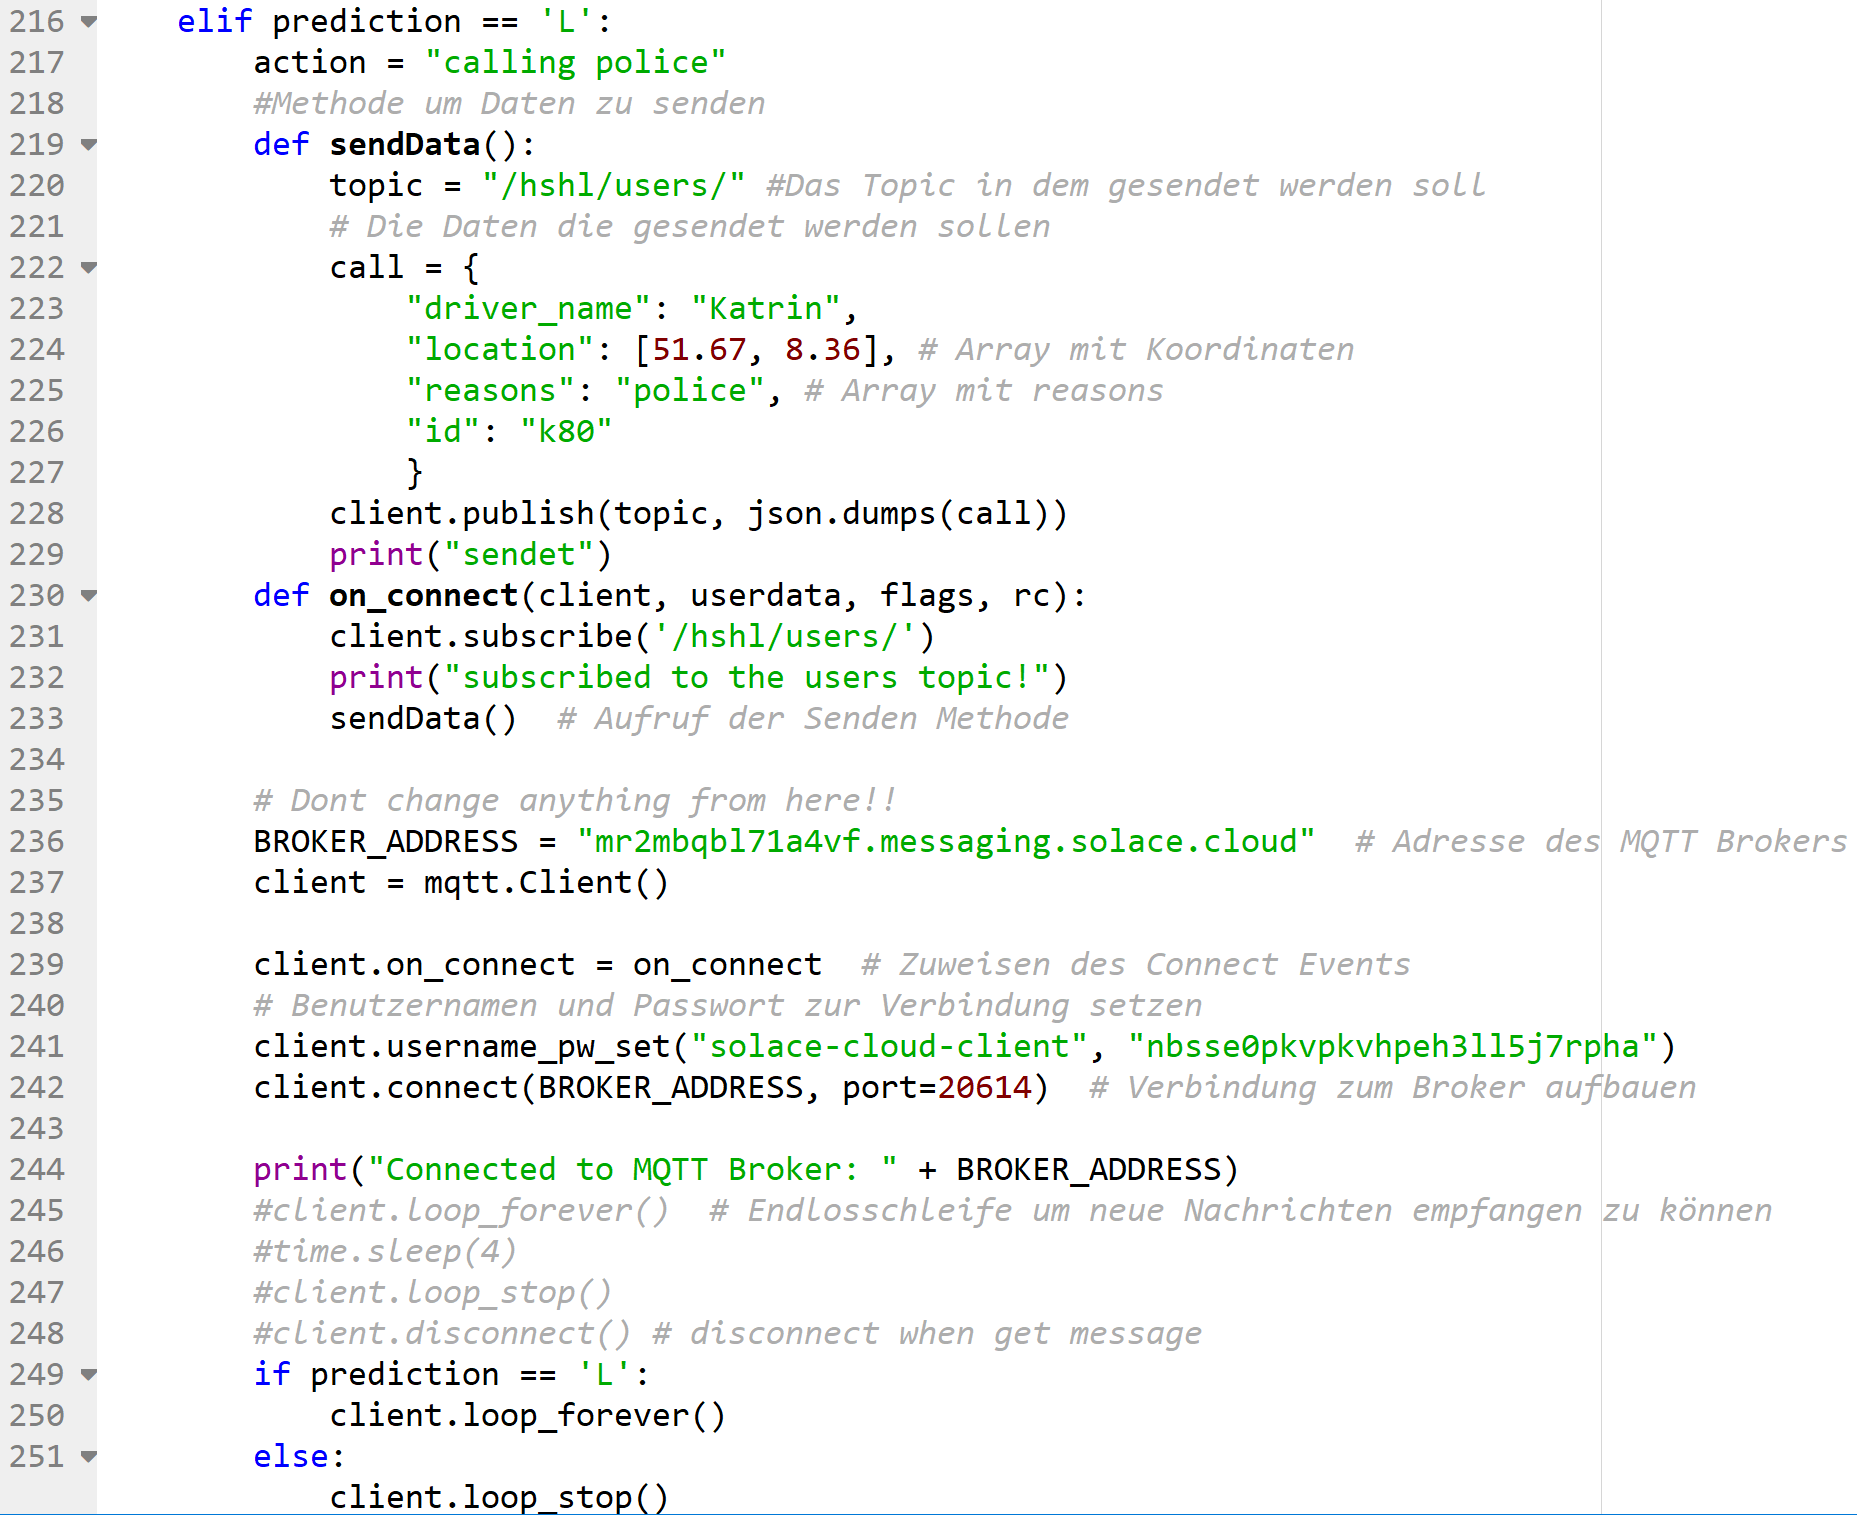
\includegraphics[scale=0.32]{images/gloewing_images/calling_police.PNG}
\caption{Connecting the system to the server.}
\label{fig:calling_police}
\end{figure}\\
In Figure \ref{fig:calling_police} is shown the connection to the server, which inside the "\textit{elif prediction == 'L'}" block. The Gesture Recognition System sends the \textit{"driver\_name"}, the \textit{"location"} of the car, the \textit{"reasons"} why the system would like to connect the server and the \textit{"id"} of the car to the server.\\



\section{Results}
\label{sec:results}

\subsection{Program Showcase}
\label{subsec:program_showcase}

Start the program by pressing the execute bottom in the individual Python development environment. After that the system will start the webcam and will use it as an input device (Figure \ref{fig:camera}).
\begin{figure}
\sidecaption
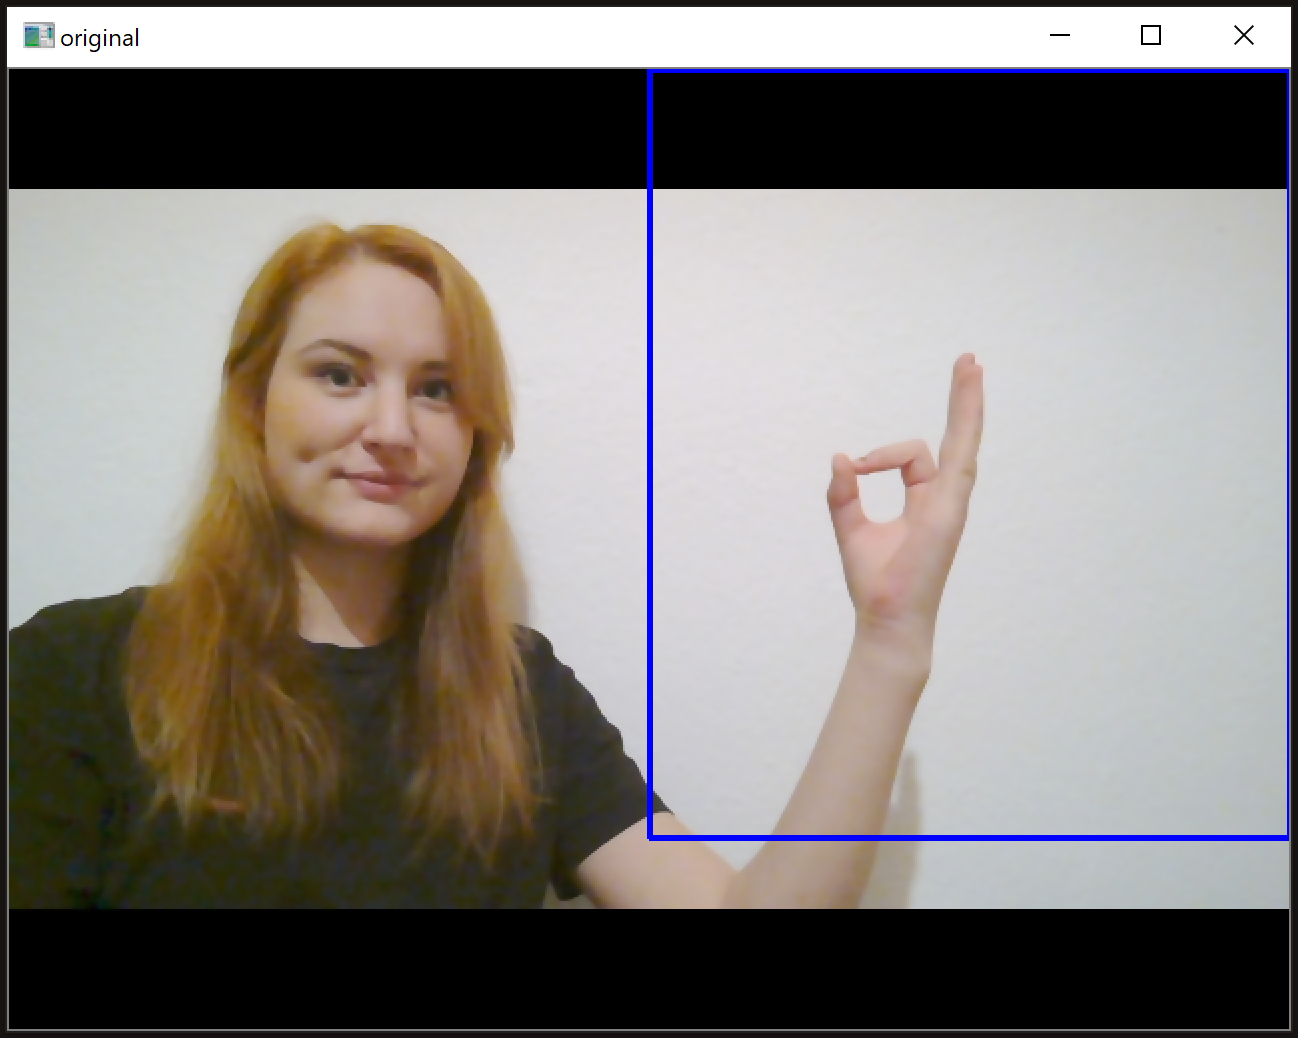
\includegraphics[scale=0.3]{images/gloewing_images/camera.PNG}
\caption{Webcam frame shown on the screen.}
\label{fig:camera}
\end{figure}\\
Next the user has to press "b" while no hand is in the blue frame, to capture the background. If this is done, the frames which are shown in Figure \ref{fig:press_b} will be opened.
\begin{figure}
\sidecaption
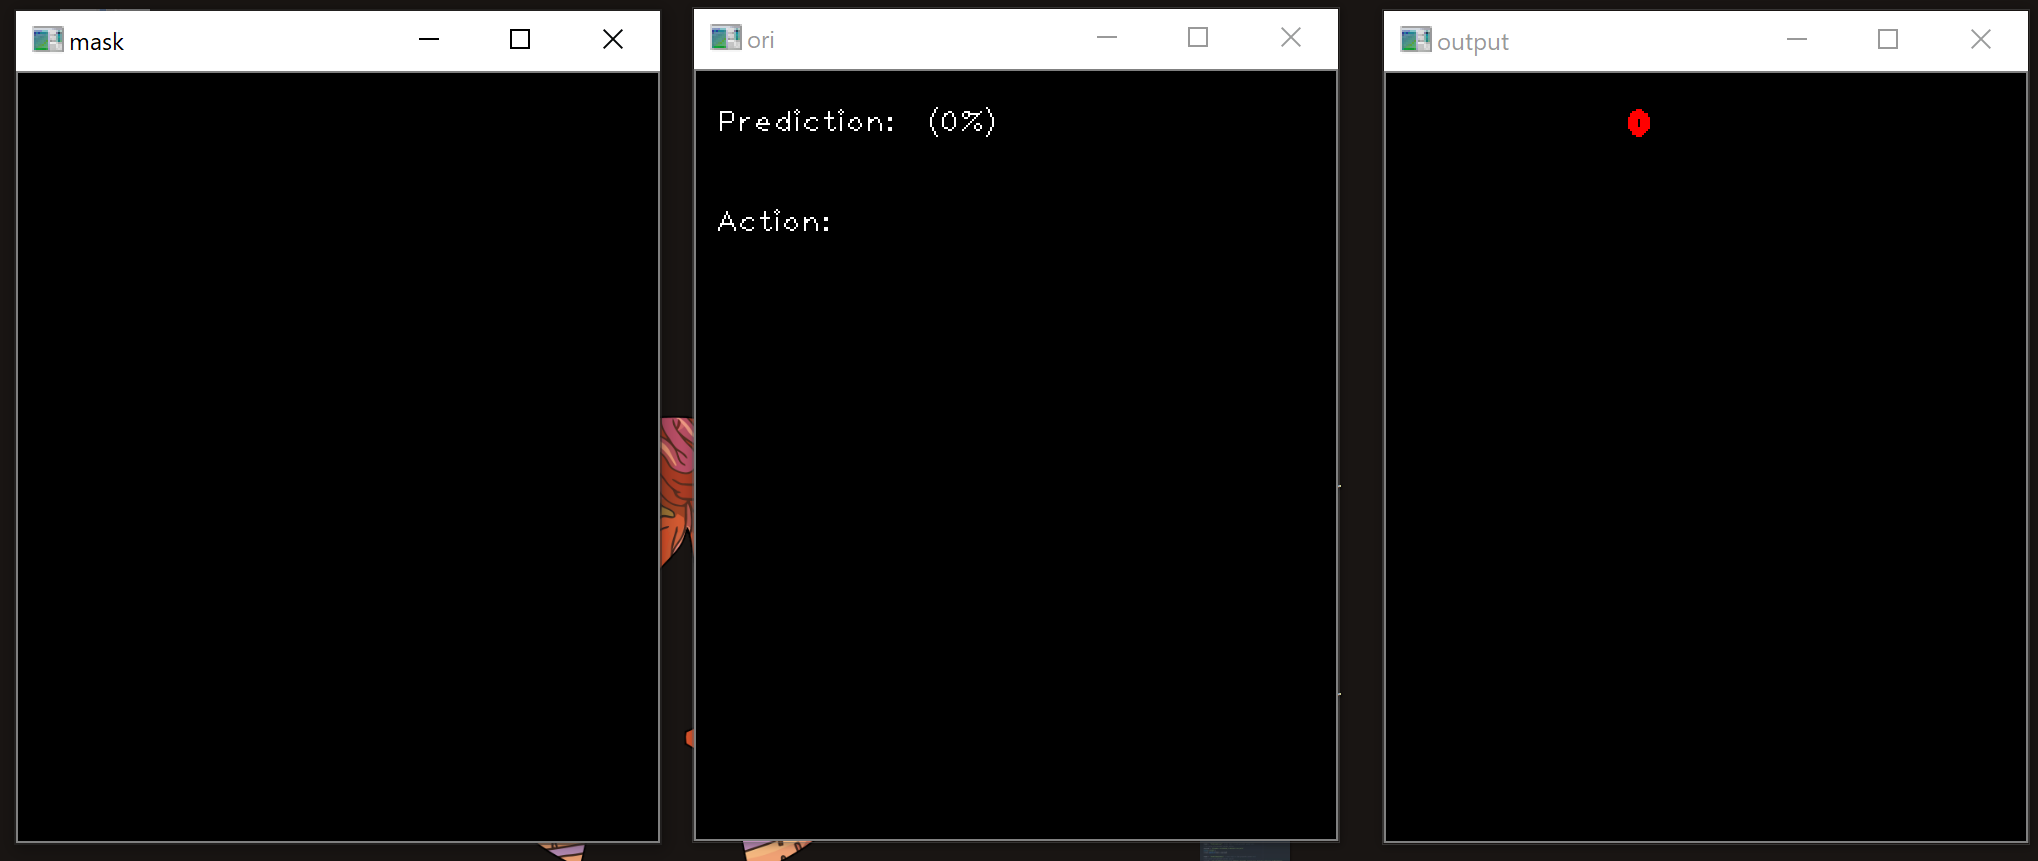
\includegraphics[scale=0.25]{images/gloewing_images/press_b.PNG}
\caption{Mask, ORI and output frame shown on the screen.}
\label{fig:press_b}
\end{figure}
\begin{figure}
\sidecaption
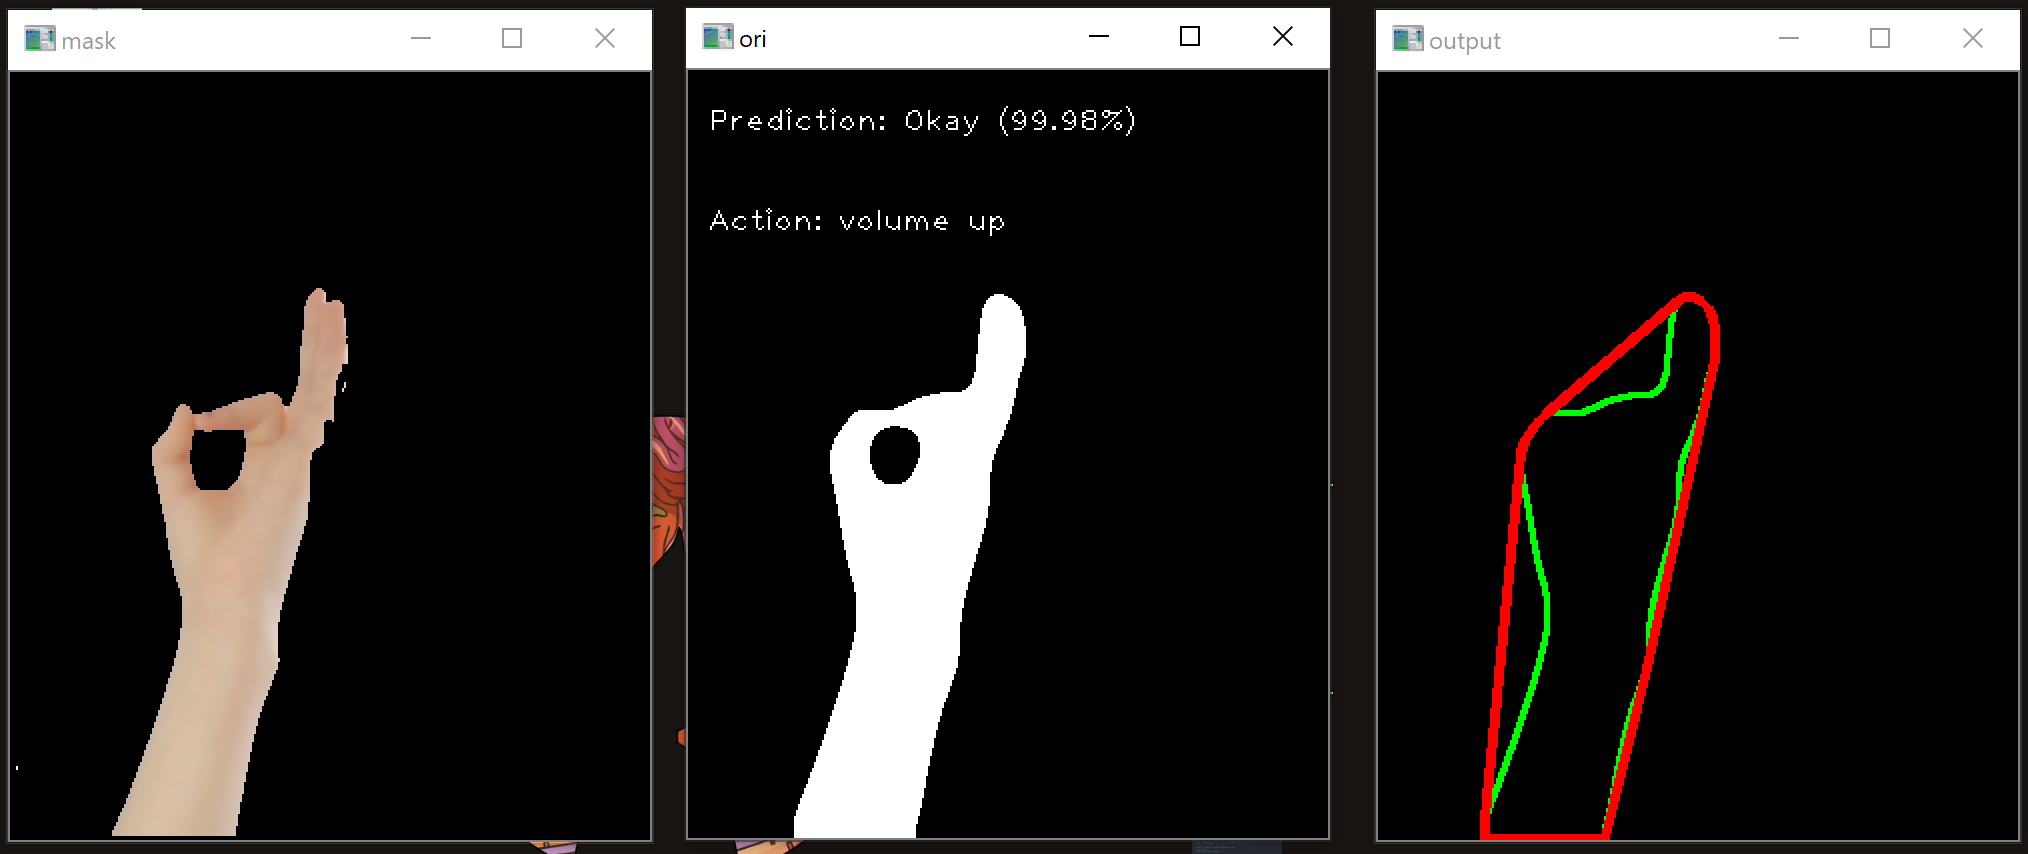
\includegraphics[scale=0.25]{images/gloewing_images/press_space.PNG}
\caption{Mask, ORI and output after showing the gesture and pressing the space-bar.}
\label{fig:press_space}
\end{figure}
\begin{figure}
\sidecaption
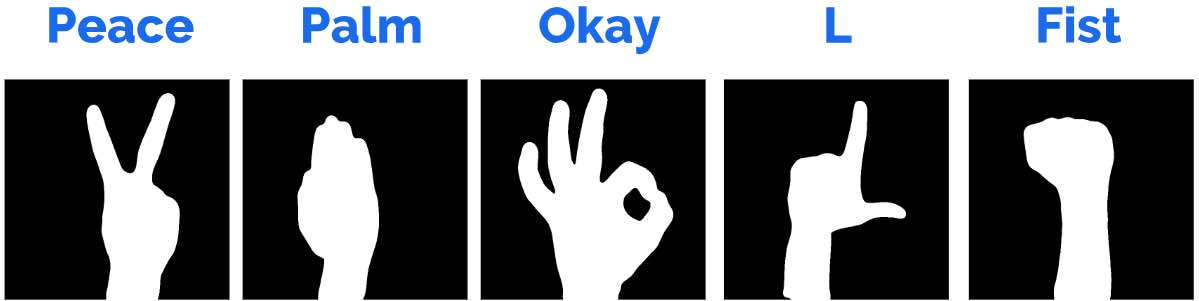
\includegraphics[scale=0.15]{images/gloewing_images/gesture_names.jpg}
\caption{Implemented gestures \cite{Brenner2018}.}
\label{fig:gesture_names}
\end{figure}\\
After that the user can show a gesture and press the space-bar to name the recognized gesture and the prediction score in the ORI frame. This is shown in Figure \ref{fig:press_space}. As it is shown, the gesture prediction is right and the probability is very high (99.98\%). The resulting action is "volume up".\\
Which kind of gestures the driver could show is presented in Figure \ref{fig:gesture_names}.\\
\\
\\
If the user would like to call the police, he or she has to present the "L" gesture and if this happens, the system will recognize the gesture and connect to the server and sends the data (see Figure \ref{fig:police_sendet}).
\begin{figure}
\sidecaption
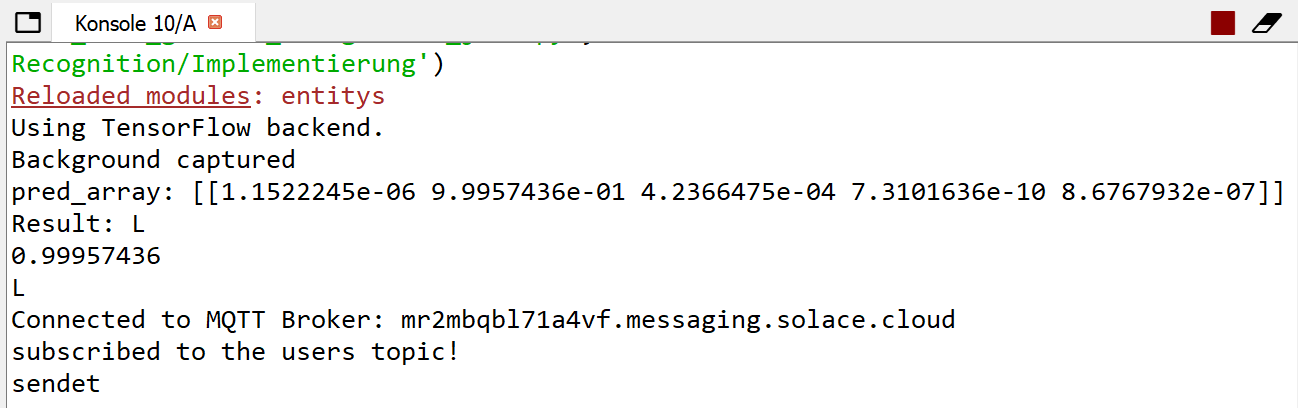
\includegraphics[scale=0.4]{images/gloewing_images/police_sendet2.PNG}
\caption{The panel is showing that the system sends data to the server.}
\label{fig:police_sendet}
\end{figure}
\begin{figure}
\sidecaption
\includegraphics[scale=0.8]{images/gloewing_images/police_empfängt.PNG}
\caption{The command prompt is showing that the server receives the data.}
\label{fig:police_empfängt}
\end{figure}\\
Figure \ref{fig:police_empfängt} shows the command prompt from the server. The request is successfully received.

\subsection{Implemented Requirements}
\label{subsec:implemented_requirements}
Each requirement, functional and non-functional, is implemented (Figure \ref{fig:requirements}).\\
There are five different hand gestures which can be recognized by this system (Figure \ref{fig:requirements}, R1), two more than determined before.\\
The "L" gesture calls the police by making a request to the server (Figure \ref{fig:requirements}, R2).\\
The requirement R3 "\textit{The system must have trained a neuronal network}" is also fulfilled. As it is described in section \ref{subsec:system} the system uses the VGG-16 Model with four additional dense layers \cite{Brenner2018}. The system is already trained by Brenner Heintz \cite{Brenner2018} in the cloud with AWS and by cross-validating his model with data from Kaggle from Benen Harrington \cite{Harrington2018}. For more information on this topic, follow the corresponding URL-Links in the references.\\
The output is the name of the gesture and is shown on the top at the ORI frame (Figure \ref{fig:requirements}, R4) including the corresponding probability and the following action of the system.\\
The system is written in Python (Figure \ref{fig:requirements}, R5) and uses the OpenCV library (Figure \ref{fig:requirements}, R7).\\
The input device for the hand gestures is the webcam (Figure \ref{fig:requirements}, R6) and the additional input device for controlling the system is the keyboard.


\section{Conclusion}
\label{sec:conclusion}
Towards the end, this Gesture Recognition System is clearly useful. Detecting the hand gesture by using the pre-trained VGG-16 model with four additional dense layers on top with B. Heintz's and B. Harrington's data sets works smooth.\\
In the introduction (section \ref{sec:introduction}) is described that tending a hardware with gestures is growing in importance in case of human machine interface. The Figure \ref{fig:statistic} shows only a \textit{projected} global gesture recognition and touchless sensing market size for the year 2020 but in section \ref{sec:relatedworks} it is proved, that there are some new gesture control systems since 2014.\\ Section \ref{sec:concept} defined the goal of the project, the requirements and the use cases.\\
The following section (section \ref{sec:implementation}) describes the used VGG-16 model in detail and some implementations like importing the necessary packages, defining the gesture names, loading the model, transforming the data, extracting the gesture, defining the corresponding actions of the well defined gestures and connecting the system to the server.\\
The results are demonstrated in section \ref{sec:results}. The program showcase (section \ref{subsec:program_showcase}) proves, that the system works and how the system works from the users point of view. The section \ref{subsec:implemented_requirements} shows that each requirement is implemented including two more hand gestures and the keyboard as one additional input.\\
It would be operative to implement this hand gesture recognition system into real cars, to control some car activities by showing hand gestures. This will helps car drivers to keep focused on the road because it is not necessary to find bottoms on the centre consol display in the car. The entries to control the car activities will be done by hand gestures. An advantage over using speech input is that if its too loud for the system to recognize what the driver said, the voice control does not work. For the gesture recognition system is loudness no problem.\\
This system is not only for cars, it can also be installed in different vehicles like trains or motor trucks.\\
Another option which can this system be a base for, is for detecting 	sign language. Some of the used gestures are already some gestures of the sign language. The \textit{fist gesture} represents an \textit{A}, the \textit{palm gesture} stands for an \textit{B}, the \textit{peace sign} represents in the sign language the letter \textbf{V} or \textit{K}, it depends on how the fingers are crossed, and the \textit{L gesture} is actually the letter \textit{L} in the sign language.\\

\newpage
\bibliographystyle{IEEEtran}
\bibliography{chapters/chapter7_katrin/chapter.bib}
